%!TEX root = thesis_proposal.tex

\section{Methodology}
\label{sec:m}

This section will first present the methodology employed by NDW to produce the prototype implementation and the one implemented by RHDHV to produce the commercial toolbox. It will then present a detailed overview of my proposed research methodology, separating the processing and the accuracy assessment procedures into two separate workflow descriptions.

NDW themselves produced a non-commercial prototype implementation, which can achieve a 3D enrichment of NWB with only a few gaps in the produced elevation profiles. Although their workflow does not have a formal documentation, I have been given a verbal description of it, as well as the output. Based on my understanding of these, their primary technique involved snapping close-by AHN3 Lidar points to the line geometries of NWB. Notable problems with the implementation included non-road points being snapped to centrelines, causing road centrelines to be extruded to overestimated elevations, in turn resulting in sudden jumps in the elevation profiles. Furthermore, no close-by points could be found for underground roads (i.e. tunnels), and strongly occluded parts of roads. For small gaps, this was resolved partially by writing an algorithm to interpolate linearly inside NWB, using the closest vertices where snapping was successful. For larger gaps, an attempt was made to resolve issues by including information from external sources semi-automatically. Neither one of these issues could be fully resolved via these approaches, hence the results of this project were only used by NDW to gain a better understanding of the problem and the expected challanges. For a reliable, commercial toolbox they subsequently commissioned an implementation from RHDHV.

RHDHV developed their implementation in parallel with the \textit{planning} of the present scientific research. I have attended NDW-RHDHV meetings, discussed the implementation directly with RHDHV, and was granted access to the codebase of the project. Understanding their implementation is crucial for this research, as it aims to both assess the accuracy of the commercial implementation, as well as, in part, base its methodology and implementation on the suspected shortcomings on the commercial implementation. First, where NWB vertices are too sparse, densification takes place and additional temporary vertices are created inside NWB line segments. Then, \textit{different} workflows are initiated for R-roads and P-roads. For P-roads (for which DTB data does not generally exist), the workflow is conceptually similar to the one in the prototype, with the notable difference of using AHN3 DTM rasters rather than the point cloud. Because AHN3 DTM rasters are badly affected by both large holes and small groups of missing pixels (due to the fixed-parameter IDW interpolation that was used to generate them), RHDHV could only make use of them by filling in the gaps of the raster using linear interpolation in a 3D TIN created from the raster pixel centres and their elevations. They overlaid the raster tiles with NWB vertices (including the dense, temporary vertices) and interpolated their elevations using bilinear interpolation inside the raster. For R-roads DTB is available, and the assumption is made by RHDHV that it is more accurate than AHN3 (or at least the stock DTM tiles generated from AHN3), to the extent where it should be the primary source of elevation data. Priority is thus given to it in the procedure, with AHN-based interpolation used only as a fallback mechanism in case DTB-based height estimation fails. The goal of the procedure is to find the DTB line segments that delineate the road edges at any given location in the NWB and deduce elevations from them. First, 2D cross-sections are constructed on NWB vertices, with each given the mean azimuth of the two NWB line segments that they are part of, and also on densified vertices, which receive azimuth values based simply on the azimuth of their parent line segments. DTB lines are then intersected with the cross-sections and for each cross-section, the closest DTB line that satisfies a relative angle condition is picked on both sides. Elevation is then first linearly interpolated inside the two chosen DTB segments to yield values exactly at their intersections with the cross-section. Then, elevation is interpolated linearly along the cross-section itself to yield the final elevation of the NWB vertex or densified temporary vertex. The angle condition is a threshold-based evaluation concerning the angle between intersected DTB lines and cross-sections and is intended to ensure that the chosen DTB segment indeed represents the edge of the current road, rather than some other feature, or the edge of another road. Hence, the assumption is made that the DTB line segments representing road edges are roughly parallel with the relevant NWB centrelines and lie close to them. Implicitly, this also assumes that NWB centrelines will lie between DTB road edges. In practice, none of these assumptions holds in general, hence a range of failsafe mechanisms needed to be implemented. Wherever the algorithm only finds a suitable DTB intersection on one side of NWB, it is only that side from which the elevation value is deduced. If no suitable intersection can be found whatsoever, the AHN3 raster-based interpolation is used instead. At NWB centreline end vertices (where no intersection exists, i.e. dead ends), the previous vertex’s elevation is simply repeated. The described methodology is illustrated in Figure \ref{fig:rhdhv}. It is worth mentioning that the RHDHV implementation deals with all non-standard input data sets (i.e. small-scale engineering models, road management datasets, etc.) by first converting them to rasters with the same specifications as AHN3 DTM tiles and mosaicking them into an output raster based on a priority list, before filling in any remaining gaps and interpolating bilinearly.

\begin{figure}[h]
    \centering
    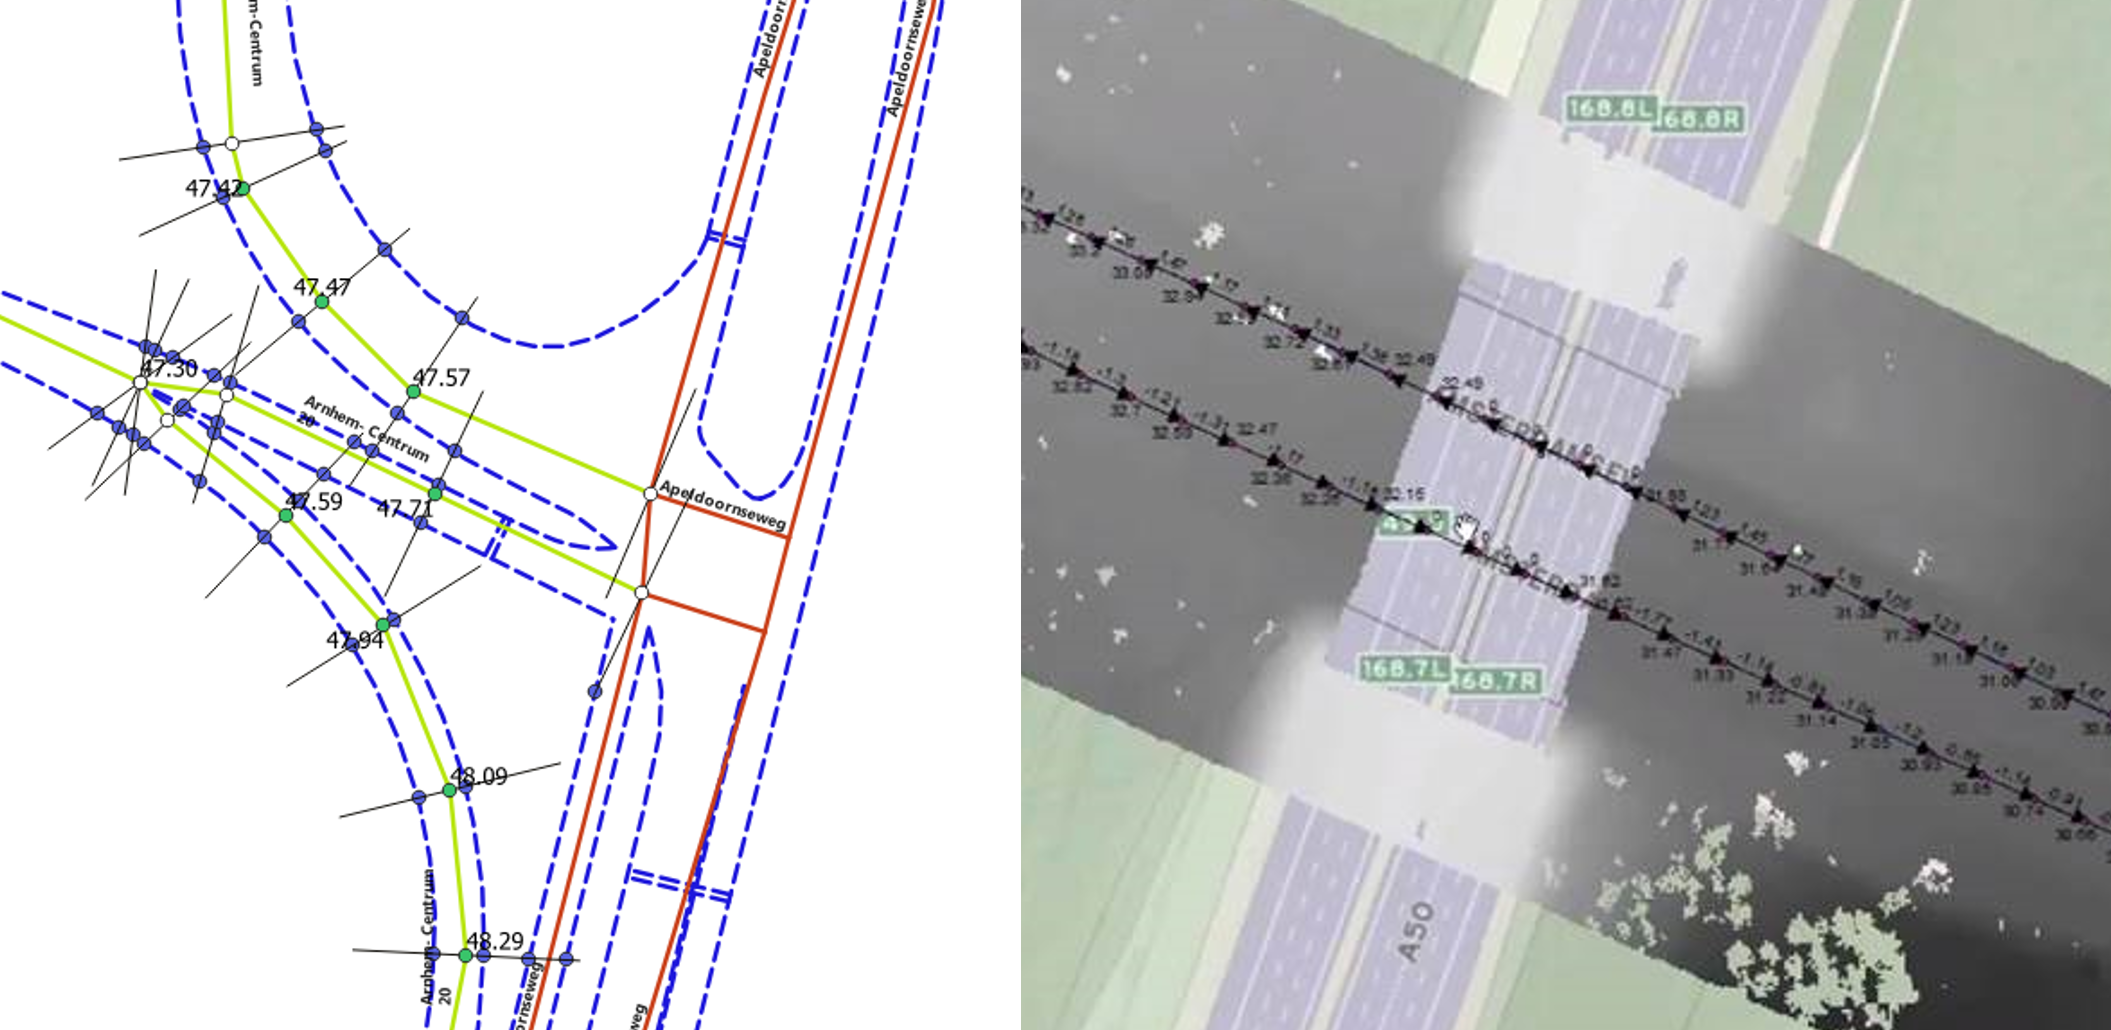
\includegraphics[width=\linewidth]{p2/figs/rhdhv_combined.png}
    \caption{Illustrations of RHDHV's commercial implementation. \textbf{Left:} The cross-sections that are constructed on NWB vertices are shown as black lines. Green circles denote those vertices where the cross section could be properly intersected with DTB \textit{verflijnen} (blue circles) and thus be given an elevation value. White circles denote where the procedure failed, and AHN raster-based interpolation was necessary. This render illustrates that in sharp bends (where the cross-section might not intersect DTB orthogonally) and close to intersections, this workflow often fails, and that P-roads are not processed in this way (they have DTB edges in this particular location only because they are close to R-roads). \textbf{Right:} AHN-based interpolation is used for P-roads, and as a fallback mechanism where DTB-based interpolation fails. The rasters are overlain with NWB to yield elevation values, and as the DSM rasters contain holes, they are patched in by pre-interpolating them before this step. In this illustration, the holes are left in to show that two types of holes generally occur: small-scale ones due to objects such as street furniture, vehicles and vegetation, and large ones that are typically due to occlusion from overlapping buildings or bridges (as in this case). The test build shown here uses AHN2 rasters.}
    \label{fig:rhdhv}
\end{figure}

There are various sources of issues that I this methodology suggests, from a scientific point of view. For instance, point cloud to raster conversion is, by definition, associated with inherent information loss (less raster cells than pixels), and further reduction in accuracy is introduced by the interpolation mechanism itself. Radial IDW was used to generate AHN3 DTM tiles, which several of the reviewed papers found to be specifically unsuitable for interpolating large-scale areas in which zones of decreased point density or gaps exist – both of which characterise ground-filtered AHN data (e.g. \cite{guo_etal_2010}). In addition, the procedure performs another layer of interpolation to infill gaps, which may further affect accuracy negatively. It is also worth mentioning that RHDHV uses bilinear interpolation inside the raster to produce NWB elevations, which is suggested by \cite{shi_etal_2005}, to be less accurate than other common methods such as bicubic. In terms of their strong prioritising of DTB for R-roads, I should remark that DTB is also a secondary source of information (it is based on procedurally combining various types of sensing into vector features), and in contrast with AHN3, neither its overall nor its local accuracy are reported in its documentation or known from elsewhere. While it no doubt contains valuable information that may benefit the overall procedure, relying on it as the sole source of elevation data may not be an approach that can guarantee the levels of accuracy needed for SWUNG2 compliance.

My proposed approach is the result of a combined understanding of concepts in related work, my own knowledge and experience relating to geomatics concepts and methods, as well as inspiration from the commercial implementation of RHDHV. The proposed workflow was built with the research questions in mind. The below summary is only a top-level description, as I expect the detailed specifications to change.

\begin{enumerate}
    \item Pre-processing
    \begin{enumerate}
        \item Keep only NWB R-roads and P-roads. Identify \textit{non-branching road segments}, henceforth referred to as \textit{NBRSs}. To identify them, first look for interconnected networks of MultiLineString objects sharing the same street name, then split off branches at intersections, always doing so in the order of decreasing angle (to ensure that a straight continuation of roads is natively preferred). Perform vertex densification for NBRS edges longer than a set distance.
        \item Keep only AHN3 points within a set distance from NWB lines. Keep classes 2 and 26 only.
        \item Keep only DTB “verflijnen”.
    \end{enumerate}
    \item Point cloud partitioning
    \begin{enumerate}
        \item For each NBRS from the previous stage, fit planes to the neighbourhood of edges and fetch points that are close to them. When selecting a final plane from candidate planes, perform a similarity check between the parameters of neighbouring planes, so that the resulting succession of planes are not oriented unrealistically with respect to each other. Determine the exact procedure and parametrisation in a way that it is not too complex computationally, but still captures most Lidar points relevant to the given NBRS (i.e. do not use conservative thresholds at this stage).
        \item Merge the sub-clouds of edges into a single sub-cloud for the NBRS and save to disk with an identifier linking it to the NBRS itself.
    \end{enumerate}
    \item Road edge identification
    \item[] To be performed on each generated NBRS (and linked sub-cloud of Lidar points).
        \begin{enumerate}
            \item Construct cross-sections on NBRS vertices (including densified vertices) and snap close-by AHN3 points to them at a pre-set sampling distance along each of them.
            \begin{enumerate}
                \item Find the dominant line parametrisations of their elevation profiles and discard non-conformant points.
                \item Disregard points separated by gaps (created by the previous step) from the main group of points representing the fitted line (close to NWB), and points outside a maximum allowed road width. The outermost points in the detected series represent the approximate local position of the road edge on each side.
                \item Disregard cross-sections where steps i. or ii. indicate that locally, NWB does not lie on the road surface as suggested by AHN3 (for instance, because the cross-section regression line does not cross the centreline in 2D).
                \item Derive mean elevations for each cross-section from the remaining points.
            \end{enumerate}
            \item The series of mean elevations (one per cross-section) is itself a 1D elevation profile. Perform outlier detection by sliding a kernel along this profile. Discard cross-sections where this operation indicated that the fitted line is significantly above the road surface. This will help eliminate cross sections corrupted by local groupings of non-road points (such as class-26 motorway signs).
            \item Assemble approximate global road edges from the two outermost Lidar points (on each side of NWB) of each cross-section kept after the pervious step.
            \item Use the left and right road edge estimates from the previous step as initial approximations in an active contour optimisation step. The constraints (energy terms): realistic horizontal distance from NWB for Dutch roads, and/or realistic distance from its own initial edge estimate, and a term “detecting” the first noticeable local change in curvature away from NWB.
            \item Select the Lidar points which lie between the optimised road contours in 2D. Thin the selected points to ensure that only the minimum point density needed to guarantee necessary accuracy remain.
            \item Insert the optimised contours into a CDT as constraints, and then the thinned Lidar points. Before each Lidar point insertion, interpolate in its location in the pre-existing CDT and compare the interpolated elevation to that of the Lidar point to make certain that it does not introduce unwanted curvature into the TIN. Conservative thresholds are appropriate at this stage, as road surfaces are expected to be flat locally.
            \item Interpolate NWB in the CDT using either linear, Laplace or natural neighbour interpolation (or some specialised variation thereof that uses a larger query zone and not just a single cell of the tessellation).
        \end{enumerate}
    \item NBRS merger
        \begin{enumerate}
            \item Re-assemble NWB from the NBRSs.
            \item Application of corrections at NWB intersections, smoothing. Yet undetermined if this will be necessary, as it depends on the final implementation. This topic is discussed below in more depth.
        \end{enumerate}
    \item DTB-based filling of large data gaps (more in this later in this section)
\end{enumerate}

Avoiding the creation of sudden jumps where NBRSs are stitched together may require special attention. In view of the above workflow, we may observe that in areas surrounding intersections, the CDT of each NBRS terminating there (or crossing it) will be constructed from roughly the same set of Lidar points (the road points). This is supported by the fact that the CDT construction step is mostly independent of the preceding cross-section-based workflow and the active contour approximation in the sense, that it works directly from the Lidar data. However, the proposed segmentation workflow inhibits the creation of identical CDTs at intersections because the edge-based selection procedure may not select the \textit{exact} same Lidar points for each NBRS that terminates at or crosses the intersection. This means that the same intersection vertex may be given different elevation values in different NBRSs, giving rise to ambiguity. Furthermore, depending on the quality of the raw output elevation profiles, some form of constrained smoothing (or other form of post-processing) may also be needed generally, not only at intersections. One solution that is applicable to both purposes in theory, is spline fitting. Using NWB vertices as control points could ensure not only continuity across intersections, but formal C\textsuperscript{1} smoothness across them and C\textsuperscript{2} everywhere else. However, this raises the question of how we should then treat the rule that the lateral position of NWB centrelines should not change, i.e. in theory the spline fitting would only have one degree of freedom.

Unfortunately, since the above procedure is specialised to reconstructing 3D road geometries within their paved extents, it is not applicable to the additional (non-scientific) requests I received from NDW regarding interpolating in the neighbourhood of roads to represent the topography of their vicinities. The specification of this request included the condition that the exact same method needs to be employed in the interpolation of the lines representing neighbourhood topography, as the one used for the extrusion of the centrelines themselves. Our CDT road models will be constrained by the road contours; hence it will be impossible to use them to extrude lines that are buffered from the centreline past road edges. To make this possible, the CDT would need to be augmented by inserting ground points outside the road edge constraints, extending the model to where the query line (buffered centreline) would lie. This would require working outside the segmented point clouds and fetching points directly from AHN3 tiles for a second time. As this direction of research does not fit into my methodology well and given that its motives are not strongly scientific, I am not planning to explore it any further in this project.

The above workflow uses concepts already discussed in the last few paragraphs in the Related work section (\ref{sec:rw}). For instance, the point cloud segmentation to decompose the problem into 2.5D sub-problems was inspired by \cite{oudeElberink_vosselman_2009} and \cite{boyko_funkhauser_2011}. The cross-section based workflow was, among others, inspired by \cite{yang_etal_2013} and the commercial implementation. The use of a CDT to represent the final surface comes from \cite{oudeElberink_vosselman_2006}. The active contour-based workflow was inspired by \cite{boyko_funkhauser_2011} and \cite{gopfert_etal_2011}, but while in previous research contours were attempted to be snapped to road curbs, my road-edge energy term will not be specialised to traditional curb geometries. It will be more general; a term that attracts the contour to the first noticeable change in curvature away from NWB.

For the accuracy assessment part of the project, the following secondary workflow is proposed:

\begin{enumerate}
    \item Pre-processing
    \item[] The initial accuracy of AHN3 Lidar points is unaffected.
    \item Point cloud partitioning
    \item[] The point density and spatial distribution of Lidar points decreases. However, these aspects will be considered in later steps, hence it is not necessary to quantify it here.
    \item Road edge identification
    \item[] The primary workflow ensures that interpolation takes place in a TIN generated from raw Lidar elevations. In view of this, the main aspects that need to be examined, in decreasing expected order of importance:
    \begin{enumerate}
        \item Local controls on accuracy (mainly point density and distribution, curvature). The distribution of the points (e.g. elevation variance) will be examined as an indicator of how successful the algorithm was in selecting road points only. As the stock ground filtering of AHN3 plays a part in this, the local distribution of the points will be considered indicative of that too.
        \item Interpolation accuracy. Will be determined via empirical methods in the sense that Monte Carlo simulations will be run on the final interpolation code to see how input errors propagate through it. Surveying control points or resorting to manual control point picking in the AHN3 point cloud are not planned to be part of the accuracy assessment procedure.
        \item For each NWB vertex, combined descriptors of the local point elevation variance, variance of NWB’s position relative to road edges and of road width. Together, these will be indicative of how successful the algorithm was at pinpointing road edges, how well that agrees with the NWB centreline, and how flat the road is between the contours. Based on this, it will be possible to detect areas where the procedure failed or performed very poorly, due to inaccuracies in the position of NWB, that of the detected edges, or for other reasons.
        \item For the same purpose as the evaluation in c. above, road point labelling completeness estimation will be performed manually while developing and tweaking the road edge optimisation workflow. This will be based on drawing approximate road locations on AHN3 rasters and overlaying them with the detected polygons comprised of the detected edges, connected at their end vertices. I may examine whether BRT road polygons can be used as a reference when estimating completeness over larger areas.
    \end{enumerate}
    \item NBRS merger
    \item[] Two important considerations: the accuracy description of repeated NWB vertices (vertices that are part of multiple NBRSs) will need to be aggregated from multiple NBRSs if the vertex’s elevation is aggregated numerically from their values. Or, as an alternative method, it may prove to be more effective to rely on the particular intersection elevation that has the highest estimated accuracy, giving it more weight in the aggregation or only using its value, and disregarding its less accurate counterparts. Furthermore, in case any form of smoothing or other type of post-processing is implemented, it will need to be possible to control how much it can adjust elevation values. Furthermore, the change will need to be recorded in the output.
\end{enumerate}

Due to the completeness problems, topological issues, and unverified accuracy of DTB as described in the Datasets and tools section (\ref{sec:td}), I did not include it in the primary workflow. Mostly because of the latter, from a scientific point of view, its elevation values cannot be used in a way that influences the point cloud-derived values, as it would prevent the estimation of output accuracy. However, there might be other uses for it that do not have this side-effect. Firstly, a DTB \textit{verflijn} is generally found close to the edges of R-roads and as a result, they may be useful as fallback road edge estimates where the 1D line-fitting-based method fails, in which case they would need to be intersected with the cross sections in 2D, much like in the commercial implementation. Secondly, in most places DTB appears to consistently represent the lines that are painted on R-roads a fixed distance from the actual edges of the asphalt. As such, where they do indeed represent these lines, they could be useful as secondary attractors in the active contour optimisation step, perhaps as a safeguard mechanism to ensure that blunders in the cross-section based initial road edge approximations do not affect the final road contours too badly. For such uses of DTB to become possible, they would first need to be pre-processed so that only the correct, edge-representative DTB lines are used (not, for instance the stop lines shown in the left image in Figure \ref{fig:dtbnwb}). Based on my preliminary research, the lateral location of DTB lines tends to agree better with AHN3 than that of NWB. Hence, NWB’s position relative to the closest DTB lines on each side could be a good estimator of local lateral inaccuracy in NWB. Furthermore, on bridges (where class 26 also contains reflections from bridges’ civil engineering structures), DTB lines may provide important first approximations of the road surface plane. Lastly, but perhaps most importantly, DTB can be used to fill large gaps such as those appearing underneath big structures covering the surfaces of R-roads, and in tunnels. Assuming the accuracy assessment workflow is implemented in a similar way as in the description above, then these locations will be characterised by extreme drops in point density, anomalous point distribution, very large CDT triangles, and as a result, low interpolation accuracy. In other words, we can use the derived accuracy to detect  where the algorithm encountered data gaps, and estimate how big the gaps are. For locations where only a few vertices are missing (e.g. a length of road covering only 10-20 metres), linear interpolation inside the elevation series is presumably reasonable, although it will need to be indicated in the output that this has taken place. Alternatively, the original interpolated values can be left in, assuming they are not outliers. However, where many such vertices are found in a succession, the program must assume the presence of a large AHN3 data gap. In such areas, DTB could be used as a fallback source of elevations, as it was augmented with land-based survey data wherever its primary photogrammetry-based workflow yielded insufficient data (therefore containing useful data inside tunnels and under occluding objects). However, its use would need to be marked semantically in these NWB output vertices because of the unknown accuracy of DTB. Furthermore, smoothing may need to be performed close to where DTB-based elevations are “patched into” the AHN3-based interpolation results – as the commercial results have already shown, in certain places there can be significant differences between DTB elevations and AHN3 elevations describing the same section of a road. Given the trial-and-error nature of implementing these additional DTB-based workflows in the overall procedure, some of them may end up in the final implementation, while others may be omitted. This is the reason why they are not included in the formal workflow description and are instead only vaguely described in this paragraph.

Testing the accuracy of the commercial implementation will take place via two different approaches. The ideal approach, which would be to enable the computation of the formal accuracy inside the commercial application by injecting additional code, are made difficult, likely impossible, by two factors. Firstly, their code is written in \textit{ArcPy}, hence the first step would be to port their entire codebase into the open-source framework that my implementation will be built in, or at least the main algorithms from it. Furthermore, this approach could never yield accuracy values for R-road elevations, because RHDHV rely on DTB for these roads, which does not have a formal accuracy description in its documentation. As a result, attempting this approach is not well justified. Hence, my first method will involve merely examining general properties of the output, such as smoothness, density of outliers and missing values. It will also involve a visual assessment of their results, including visual comparisons with the AHN3 point cloud and my own results, particularly in difficult environments. The second approach will involve deriving errors and RMSE values \textit{relative} to my own results. Making this comparison will indicate where the commercial results diverge from the ranges of plausible values, as specified by the uncertainty ranges in my output. Where their output falls outside these ranges of uncertainty – which could be examined visually by plotting the differences on the NWB centrelines 2D – I will examine the two results side-by-side, along with AHN3 and DTB, and attempt to explain the differences scientifically. 